%% This is an example first chapter.  You should put chapter/appendix that you
%% write into a separate file, and add a line \include{yourfilename} to
%% main.tex, where `yourfilename.tex' is the name of the chapter/appendix file.
%% You can process specific files by typing their names in at the 
%% \files=
%% prompt when you run the file main.tex through LaTeX.
\chapter{Direct Methods for Pursuit-Evasion Games}\label{chp:app}
There are a variety of methods by which pursuit-evasion games can be solved. These methods can be divided into two major categories. The first is indirect methods such as HJB-Isaacs equations. Claire Tomlin has carried out a number of interesting projects involving indirect methods of solving pursuit-evasion games \cite{tomlin1,tomlin2}. The second method of solving pursuit-evasion games is called direct methods. This chapter will explore two such direct methods. The first method is applying dynamic programming in the case that the pursuit-evasion game is a boundary value problem (BVP). Bardi, Falcone, and Soravia describe a method they use to solve a one-dimensional pursuit-evasion game in "Fully Discrete Schemes for the Value Function of Pursuit-Evasion Games" \cite{bardi2}. A type of Rapidly-exploring Random Tree(RRT) algorithm called $\textnormal{RRT}^*$ forms the basis of the second method. In "Incremental Sampling-Based Algorithms for a Class of Pursuit-Evasion Games", Karaman and Frazzoli describe how $\textnormal{RRT}^*$ can be used to solve pursuit-evasion games.  

\section{One-Dimensional Boundary Value Problems}\label{1dbvp}

An attempt to solve pursuit-evasion games by dynamic programming was made by Martino Bardi, Maurizio Falcone, and Pierpaolo Soravia in the 1990's. In their paper, "Fully Discrete Schemes for the Value Function of Pursuit-Evasion Games," Bardi, Falcone, and Soravia present a method for solving pursuit-evasion games by discretizing the state space of a boundary value problem \cite{bardi2}. The first step in their scheme is to discretize the bounded state space. This bounded state space $P$ is divided into a number of simplexes ${S_j}$ that cover the entirety of the state space without overlapping. The vertices of these simplexes are the $N$ discretized state nodes $x_i$. Furthermore, all states within the bounded state can be accounted for as a convex combination of the state nodes in $S_j$ or:
\begin{equation}
x= \sum_{i=1}^{N} \lambda_i x_i \textnormal{ where } \lambda_i \ge 0,  \sum_{i=1}^{N}\lambda_i=1,\lambda_i = 0 \textnormal{ if } x_i\notin S_j
\end{equation}
The state space is further discretized by adding points $z_i(a,b) \equiv x_i+hf(x_i,a,b) \in Q^*$, where $h$ is some time step strictly greater than 0. These points are used to determine the optimal controls from each of the discretized nodes.

\begin{figure}
\centering
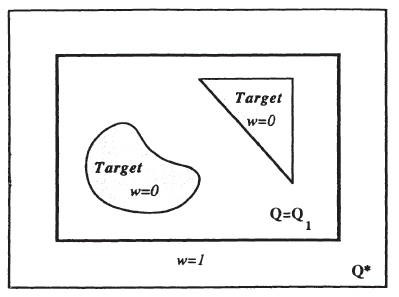
\includegraphics[scale=1]{bvpregions}
\caption{A state space divided into capture($w=0$),escape($w=1$), and regions of play($Q=Q_1$) \cite{bardi2}}
\label{bvpregions}
\end{figure}
The discretized state space is then divided into regions such as those in \Cref{bvpregions}. For this problem, $\mathscr{T}$ denotes the nodes in the target region and is a subset of the nodes in $Q$. The target region is the area in which the pursuer captures the evader. $Q_1$ is the region of play and contains all nodes in $Q$ that are not in the target region or the escape region. The escape region is denoted by $Q_2$ and may contain nodes in $Q$ and $R^M$, where $R^M$ is the boundary of the bounded state space. All the nodes in the escape region represent states in which it is assumed that the evader has avoided capture by the pursuer. A common division of the state space is to set $\mathscr{T}=$ origin, $Q_1 = Q$, and $Q_2 = R^M$. The discretization of the state space results in a discrete version of the Hamilton-Jacobi-Isaacs equation for the boundary value problem(HJD):
\begin{align}
  & w(x)  =  \sum_j\lambda_jw(x_j) && \textnormal{ if } x = \sum_j\lambda_jx_j \label{dbvp1} \\
  & w(x_i)  =  \gamma\underset{b}{\operatorname{max \textnormal{ } }}\underset{a}{\operatorname{min \textnormal{ }}} w(x_i +hf(x_i,a,b))+1-\gamma && \textnormal{ if } x_i \in Q\textbackslash \mathscr{T} \label{dbvp2} \\
  & w(x_i) = 1 && \textnormal{ if } x_i \in Q_2\textbackslash Q \label{dbvp3} \\
  & w(x_i) = 0 && \textnormal{ if } x_i \in (\mathscr{T} \cap Q) \cup (R^M \textbackslash Q_2) \label{dbvp4} \\
  & \textnormal{where } \gamma = e^{-h} \label{dbvp5}
\end{align}    


Since the HJD is completely discretized into a finite number of states, it can easily be seen that by using dynamic programming $w(x_i)$ can be solved for any initial condition $x_0$. Furthermore, in a previous paper by Bardi and Soravia, "Hamilton-Jacobi equations with singular boundary conditions on a free boundary and applications to differential games,"\cite{bardi1} they are able to prove that the continuous boundary value problem:
\begin{equation}\label{eqn1}
v(x) + \underset{b \in B }{\operatorname{min \textnormal{ }}}\underset{a \in A}{\operatorname{max}}{-f(x,a,b)\cdot Dv(x)-1}=0 \textnormal{ in } R^M\textbackslash \mathscr{T} \equiv \mathscr{T}^C,
\end{equation}
has a unique bounded viscosity solution $v$ that meets the natural Dirichlet boundary condition:
\begin{equation}\label{eqn2}
v(x) = 0 \textnormal{ for } x \in \delta \mathscr{T},
\end{equation}
if $v$ is continuous. They are further able to characterize this viscosity solution as:
\begin{equation}\label{eqn3}
v(x) \equiv 
\begin{cases}
1-e^{-\textnormal{T}(x)}, & \textnormal{ if T}(x) < + \infty,\\
1, & \textnormal{ if T}(x) = + \infty.
\end{cases}
\end{equation}
Denoting $w_n$ as the unique solution to the HJD, $Q^n$ as the discretization of the state space, $h_n$ as the time step, and $|f(x_i,a,b)| \leq M_f$, Bardi, Falcone, and Soravia show that $w_n$ will converge to the unique bounded viscosity solution $v$ as $Q^n$ and $h_n$ become infinitely small. This is presented in: 
\begin{theorem}[Convergence of Bounded Viscosity Solution \cite{bardi2}]\label{dbvpt}
Assume $|f(x,a,b)-f(y,a,b)| \leq L|x-y|$ for all $x,y,a,b$; $|f(x_i,a,b)| \leq M_f$ for all $x \in \delta$T and all $a,b$; T is the closure of an open set with Lipschitz boundary ; $(Q^n,h_n)$ is an admissible sequence ; there is a bounded continuous viscosity solution $v$ of \Cref{eqn1,eqn2}. Then $w_n$ converge to $v$ as $n \rightarrow \infty$, uniformly on any compact set of $R^M$.   
\end{theorem}
In order to demonstrate the ability of these discretized boundary value problems, Bardi, Falcone, and Soravia implemented the system of \Cref{dbvp1,dbvp2,dbvp3,dbvp4,dbvp5} with simple one-dimensional pursuit-evasion games. The results of these games can be seen in \Cref{bvpresults} \cite{bardi2}.
\begin{figure}[h!]
\centering
\begin{subfigure}[t]{0.475\textwidth}
	\centering
	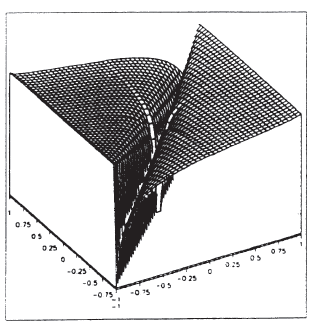
\includegraphics[width=\textwidth]{bvpresult1}
	\caption{Approximate value function when $v_1 = 1$, $v_2 = 1$}
	\label{bvpresult1}
\end{subfigure}
\hfill
\begin{subfigure}[t]{0.475\textwidth}
	\centering
	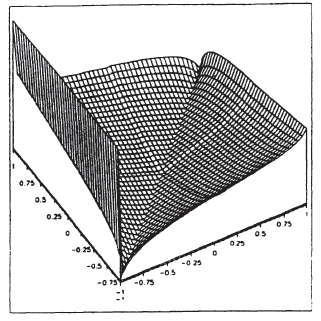
\includegraphics[width=\textwidth]{bvpresult2}
	\caption{Approximate value function when $v_1 = 5$, $v_2 = 1$}
	\label{bvpresult2}
\end{subfigure}
\caption{Results for one-dimensional pursuit-evasion games \cite{bardi2}}
\label{bvpresults}
\end{figure}
   
Bardi, Falcone, and Soravia's discrete method of solving pursuit-evasion games offers a number of advantages and disadvantages. As given in \Cref{dbvpt}, their method has the advantage of being mathematically sound. Since they focus on solving pursuit-evasion games with continuous viscosity solutions, they are able to prove that these games converge to a guaranteed optimal solution under certain conditions. A major disadvantage that arises from this is that the method does not guarantee convergence to an optimal solution if barriers or other factors that break the continuity of the solution exist. The restriction to a compact state space can also be problematic. Given too small of a state space the method might omit potential solutions that require leaving the state space. For example, given a pursuer with greater speed but less maneuverability it has been shown that an optimal strategy may require the pursuer to increase the distance between itself and the evader before making the capture \cite{isaacs}. Under these conditions the discrete boundary value problem may determine that under optimal control the evader can escape while in reality the pursuer has an optimal strategy that results in the capture of the evader.

The simple solution to this problem is to increase the state space. However, as the state space increases either the discretization must decrease or the number of discrete state nodes increases. This can be problematic when the state space encompasses a number of dimensions $d$ that are evenly discretized into $n$ states resulting in a total of $n^d$ state nodes. In this case, any increase in the discretization of the state space results in order $d$ polynomial growth of the state nodes. When $d$ is large this is called the curse of dimensionality. Bardi, Falcone, and Soravia tested their algorithm for solving discrete boundary value problems on a state space composed of 1849 nodes. Given a state of just the x and y position of both the pursuer and the evader with each dimension discretized into twenty discrete values would result in a state space with a size of $20^4 = 1.6 \times 10^5$. This method is unable to handle even moderately complex problems with a few degrees of freedom. 

\section{RRT*}
Besides dynamic programming, other methods have been used to solve pursuit-evasion games. Sertac Karaman and Emilio Frazzoli use a special version of Rapidly-exploring Random Tree (RRT) algorithm called $\textnormal{RRT}^*$ and Stackelberg strategies to solve pursuit-evasion games in "Incremental Sampling-Based Algorithms for a Class of Pursuit-Evasion Games" \cite{karaman}. Due to the edge updating scheme used by $\textnormal{RRT}^*$, this method can be effectively used as a shortest path algorithm. Karaman and Frazzoli use this method to determine the shortest path to a goal region for an evader without being caught by multiple pursuers.

The $\textnormal{RRT}^*$ algorithm is the cornerstone to Karaman and Frazzoli's ability to solve this pursuit-evasion problem. This algorithm can be used to determine the optimal shortest path as the number of iterations it is run for approaches infinity. To start the algorithm, a tree $G$ composed of vertices and edges $(V,E)$ is initialized to a single vertex at the vehicle's initial position $z_{init}$. Next, a single point $z_{rand}$ is randomly sampled from the entirety of the continuous state space $X$. The nearest vertex $z_{nearest}$ to $z_{rand}$ is then determined. A trajectory $x_{new}$ between $z_{nearest}$ and $z_{init}$ is formulated along with the controls $u_{new}$ required to traverse the trajectory. If $z_{nearest}$ can be reached within some time $t_{max}$ then $t_{new}$ takes on the time required to traverse $x_{new}$ to reach $z_{init}$. Otherwise, $t_{new} = t_{max}$. A new vertex $z_{new}$ is now determined by following $x_{new}$ for $t_{new}$. If $x_{new}$ is obstacle free, then $z_{new}$ is added to the list of vertices $V$. 

If the edge between $z_{new}$ and $z_{nearest}$ was added to the list of edges $E$, then this step along with the preceding steps would characterize the RRT algorithm. However, what makes $\textnormal{RRT}^*$ special is the next two steps in determining edges. First, within some radius all the nearby vertices, $Z_{near}$, to $z_{new}$ are used to determine the edge which reaches $z_{new}$ in optimal time $c_{min}$. The edge between $z_{new}$ and the optimal vertex $z_{min}$ is then added to $E$. Secondly, all the nearby vertices that are not $z_{min}$ are tested to determine if they can be reached in a more optimal time through $z_{new}$. If this is the case then the edge between $z_{new}$ and the vertex $z_{near}$ is added to $E$ while the edge between $z_{near}$ and the original parent, or vertex that connected $z_{near}$ to $z_{init}$, is removed. This algorithm can be viewed in detail in \Cref{RRTalg,extend} \cite{karaman}. 
  
The last two steps of $\textnormal{RRT}^*$ are especially important because they convey upon the algorithm the eventuality of optimality that is not present in RRT. If the vertices defined as nearby are all the vertices within a ball of volume $\gamma \dfrac{\textnormal{log }n}{n}$ centered at $z_{new}$ and  $n = |V|$, then $\textnormal{RRT}^*$ will converge to optimality under the conditions of \Cref{RRTopt} given that $\mu(\cdot)$ is the Lebesgue measure.
\begin{theorem}[Asymptotic Optimality of $\textnormal{RRT}^*$ \cite{karaman}]\label{RRTopt}
If $\gamma > 2^d(1+1/d)\mu(X \backslash Xi_{obs})$, the event that for any vertex $z$ that is in the tree in some finite iteration $j$ the $\textnormal{RRT}^*$ algorithm converges to a trajectory that reaches $z$ optimally, i.e., in time $T^*(z)$, occurs with probability one. Formally,
\begin{align*}
&\mathbb{P}(\{\lim\limits_{i \rightarrow \infty}T(z)[i+j] = T^*(z),   \forall z \in V[j]\}) = 1, && \forall j \in \mathbb{N}.
\end{align*}   
\end{theorem}

\begin{algorithm}
\caption{$\textnormal{RRT}^*$ \cite{karaman}}\label{RRTalg}
\begin{algorithmic}[1]
	\State $V \leftarrow {z_{init}}; E \leftarrow \null; i \leftarrow 0;$
	\While{ $i<N$} \do{}
		\State $G \leftarrow (V,E);$
		\State $z_{rand} \leftarrow \textnormal{Sample}(i);$
		\State $(V,E,z_{new}) \leftarrow \textnormal{Extend}(G,z_{rand});$
		\State $i \leftarrow i +1;$
	\EndWhile
\end{algorithmic}
\end{algorithm} 

\begin{algorithm}
\caption{$\textnormal{Extend}(G,z)$ \cite{karaman}}\label{extend}
\begin{algorithmic}[1]
	\State $V' \leftarrow V; E' \leftarrow E;$
	\State $z_{nearest} \leftarrow \textnormal{Nearest}(G,z);$
	\State $(x_{new},u_{new},t_{new}) \leftarrow \textnormal{Steer}(z_{nearest},z); z_{new} \leftarrow x_{new}(t_{new});$
	\If{ $\textnormal{ObstacleFree}(x_{new})$}
		\State $V' \leftarrow V' \cup \{z_{new}\};$
		\State $z_{min} \leftarrow z_{nearest}; c_{min} \leftarrow T(z_{new});$
		\State $Z_{nearby} \leftarrow \textnormal{Near}(G,z_{new},|V|);$
		\For{ all $z_{near} \in Z_{nearby}$} \do{}
			\State $(x_{near},u_{near},t_{near}) \leftarrow \textnormal{Steer}(z_{near},z_{new});$
			\If{ObstacleFree$(x_{near})$ and $x_{near}(t_{near})=z_{new}$ and $T(z_{near}) + \textnormal{EndTime}(x_{near})< T(z_{new})$}
				\State $c_{min} \leftarrow T(z_{near})+\textnormal{EndTime}(x_{near});$
				\State $z_{min} \leftarrow z_{near};$
			\EndIf
		\EndFor
		\State $E' \leftarrow E' \cup \{(z_{min},z_{new})\};$
		\For{ all $z_{near} \in Z_{nearby} \ \{z_{min}\}$} \do{}
			\State $(x_{near},u_{near},t_{near}) \leftarrow \textnormal{Steer}(z_{new},z_{near});$
			\If{ ObstacleFree$(x_{near})$ and $x_{near}(t_{near})=z_{near}$ and $T(z_{near})>T(z_{new})+\textnormal{EndTime}(x_{near})$}
				\State $z_{parent} \leftarrow \textnormal{Parent}(z_{near});$
				\State $E' \leftarrow E' \ \{(z_{parent},z_{near})\};E' \leftarrow E' \cup \{(z_{new},z_{near})\};$
			\EndIf
		\EndFor
		\Else
			\State $z_{new} = \textnormal{NULL};$
	\EndIf
	\State
	\Return $G' = (V',E',z_{new})$
\end{algorithmic}
\end{algorithm}

Karaman and Frazzoli further apply the $\textnormal{RRT}^*$ algorithm to solve pursuit-evasion games. In order to do this, they implement a Stackelberg strategy in which the evader first choses its controls and then the pursuers  follow the evader by choosing their controls to counter the strategy of the evader. These types of strategies provide for a worst case scenario for the evader. Therefore, if the $\textnormal{RRT}^*$ pursuit-evasion algorithm finds a winning strategy for the evader this strategy will always result in a win for the evader no matter what strategy the pursuers choose.

The pursuit-evasion algorithm modifies upon $\textnormal{RRT}^*$ by creating trees for both the evader $G_e$ and the pursuer $G_p$. Besides creating two separate trees, the pursuit-evasion algorithm also checks all the nearby vertices of the other player. If the new evader vertex can be reached in less time by a nearby pursuer vertex or a new pursuer vertex can reach nearby evader vertices in less time, then those evader vertices along with their connecting edges are removed from $G_e$. This algorithm can be examined in detail in \Cref{RRTpealg} \cite{karaman}.
         
\begin{algorithm}
\caption{Pursuit-Evasion $\textnormal{RRT}^*$ \cite{karaman}}\label{RRTpealg}
\begin{algorithmic}[1]
	\State $V_e \leftarrow {x_{e,init}}; E_e \leftarrow \null; V_p \leftarrow {x_{p,init}}; E_p \leftarrow \null; i \leftarrow 0;$
	\While{ $i<N$} \do{}
		\State $G_e \leftarrow (V_e,E_e);G_p \leftarrow (V_p,E_p)$
		\State $z_{e,rand} \leftarrow \textnormal{Sample}_e(i);$
		\State $(V_e,E_e,z_{e,new}) \leftarrow \textnormal{Extend}_e(G_e,z_{e,rand});$
		\If{$z_{e,new} \neq \textnormal{NULL}$}
			\State $Z_{p,near} \leftarrow \textnormal{NearCapture}_e(G_p,z_{e,new},|V_p|);$
			\For{ all $z_{p,near} \in Z_{p,near}$} \do{}
				\If{Time$(z_{p,near}) \leq \textnormal{Time}(z_{e,new})$}
					\State Remove$(G_e,z_{e,new});$
				\EndIf
			\EndFor
		\EndIf
		\State $z_{p,rand} \leftarrow \textnormal{Sample}_p(i);$
				\State $(V_p,E_p,z_{p,new}) \leftarrow \textnormal{Extend}_p(G_p,z_{p,rand});$
				\If{$z_{p,new} \neq \textnormal{NULL}$}
					\State $Z_{e,near} \leftarrow \textnormal{NearCapture}_p(G_e,z_{p,new},|V_e|);$
					\For{ all $z_{e,near} \in Z_{e,near}$} \do{}
						\If{Time$(z_{p,new}) \leq \textnormal{Time}(z_{e,near})$}
							\State Remove$(G_e,z_{e,near});$
						\EndIf
					\EndFor
				\EndIf
		\State $i \leftarrow i +1;$
	\EndWhile
	\State
	\Return $G_e,G_p$
\end{algorithmic}
\end{algorithm}

In order to demonstrate the abilities of the pursuit-evasion $\textnormal{RRT}^*$, Karaman and Frazzoli implement this algorithm on two different examples. In the first example, simplified dynamics are used. For the evader, the dynamics are:
\begin{equation*}
\dfrac{d}{dt}x_e(t) = \dfrac{d}{dt}\left[ \begin{array}{c}
x_{e,1}(t) \\
x_{e,2}(t) \end{array} \right] = u_e(t) = \left[ \begin{array}{c}
u_{e,1}(t) \\
u_{e,2}(t) \end{array} \right],
\end{equation*}
with $\|u_e(t)\|_2 \leq 1$, while the pursuers have the following dynamics:
\begin{equation*}
\dfrac{d}{dt}x_p(T) = \dfrac{d}{dt}\left[ \begin{array}{c}
x_{p_1}(t) \\
x_{p_2}(t) \\
x_{p_3}(t) \end{array} \right] = \dfrac{d}{dt}\left[ \begin{array}{c}
x_{p_1,1}(t) \\
x_{p_1,2}(t) \\
x_{p_2,1}(t) \\
x_{p_2,2}(t) \\
x_{p_3,1}(t) \\
x_{p_3,1}(t) \end{array} \right] =
\left[ \begin{array}{c}
u_{p_1}(t) \\
u_{p_2}(t) \\
u_{p_3}(t) \end{array} \right] = \left[ \begin{array}{c}
u_{p_1,1}(t) \\
u_{p_1,2}(t) \\
u_{p_2,1}(t) \\
u_{p_2,2}(t) \\
u_{p_3,1}(t) \\
u_{p_3,1}(t) \end{array} \right],
\end{equation*}                   
with $\|u_{p_1}(t)\|_2 \leq 1$, $\|u_{p_2}(t)\|_2 \leq 0.5$, and $\|u_{p_3}(t)\|_2 \leq 0.5$. The second example uses Dubins dynamics where the evader can be modeled by the following differential equations:
\begin{align*}
& x_e(t) = [x_{e,1}(t),x_{e,2}(t),x_{e,3}(t),x_{e,4}(t),x_{e,5}(t)]^T , & \\
& f(x_e(t),u_e(t)) = [v_e \textnormal{cos}(x_{e,3}(t)),v_e \textnormal{sin}(x_{e,3}(t)),u_{e,1}(t),x_{e,5}(t),u_{e,2}(t)]^T , &\\
& \dot{x}_e(t) = f(x_e(t),u_e(t)), & \\
& v_e = 1, |u_{e,1}(t)| \leq 1, |u_{e,2}(t)| \leq 1, |x_{e,5}| \leq 1. &
\end{align*} 
The pursuer also follows Dubins dynamics with the following differential equations:
\begin{align*}
& x_p(t) = [x_{p,1}(t),x_{p,2}(t),x_{p,3}(t),x_{p,4}(t),x_{p,5}(t)]^T , & \\
& f(x_p(t),u_p(t)) = [v_p \textnormal{cos}(x_{p,3}(t)),v_p \textnormal{sin}(x_{p,3}(t)),u_{p,1}(t),x_{p,5}(t),u_{p,2}(t)]^T , &\\
& \dot{x}_p(t) = f(x_p(t),u_p(t)), & \\
& v_p = 2, |u_{p,1}(t)| \leq 1/3, |u_{p,2}(t)| \leq 1, |x_{p,5}| \leq 1. &
\end{align*}
The results of these examples can be seen in \Cref{rrtfig,rrtobsfig,rrtdubinsfig} \cite{karaman}.   
\begin{figure}
\centering
\begin{subfigure}[b]{0.475\textwidth}
	\centering
	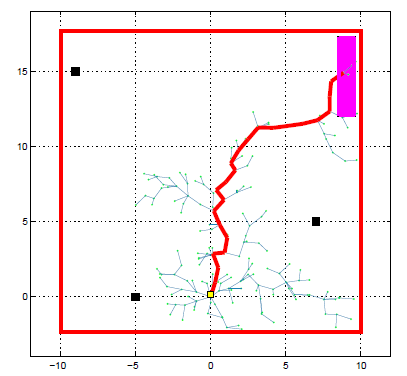
\includegraphics[width=\textwidth]{rrt500}
	\caption{500 iterations }
	\label{rrt500}
\end{subfigure}
\hfill
\begin{subfigure}[b]{0.475\textwidth}
	\centering
	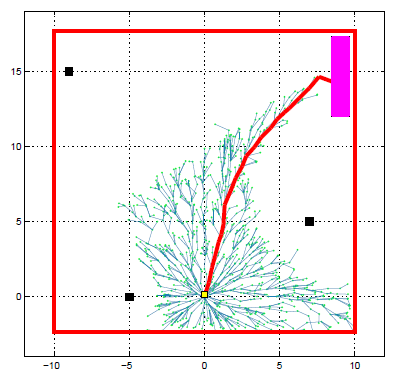
\includegraphics[width=\textwidth]{rrt3000}
	\caption{3000 iterations}
	\label{rrt3000}
\end{subfigure}
\vskip\baselineskip
\begin{subfigure}[b]{0.475\textwidth}
	\centering
	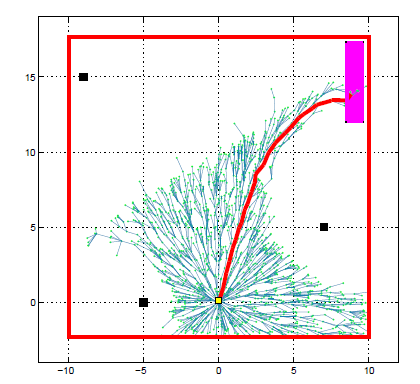
\includegraphics[width=\textwidth]{rrt5000}
	\caption{5000 iterations}
	\label{rrt5000}
\end{subfigure}
\quad
\begin{subfigure}[b]{0.475\textwidth}
	\centering
	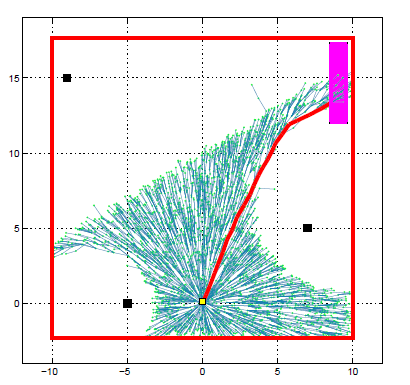
\includegraphics[width=\textwidth]{rrt10000}
	\caption{10000 iterations}
	\label{rrt10000}
\end{subfigure}
\caption{Pursuit-Evasion $\textnormal{RRT}^*$ at various iterations \cite{karaman}}
\label{rrtfig}
\end{figure}

\begin{figure}
\centering
\begin{subfigure}[b]{0.475\textwidth}
	\centering
	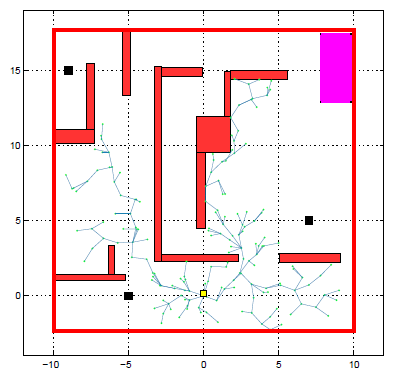
\includegraphics[width=\textwidth]{rrtobs500}
	\caption{500 iterations}
	\label{rrtobs500}
\end{subfigure}
\hfill
\begin{subfigure}[b]{0.475\textwidth}
	\centering
	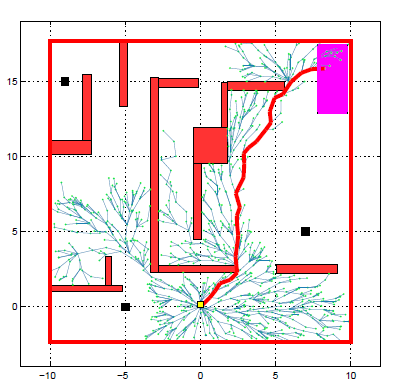
\includegraphics[width=\textwidth]{rrtobs3000}
	\caption{3000 iterations}
	\label{rrtobs3000}
\end{subfigure}
\vskip\baselineskip
\begin{subfigure}[b]{0.475\textwidth}
	\centering
	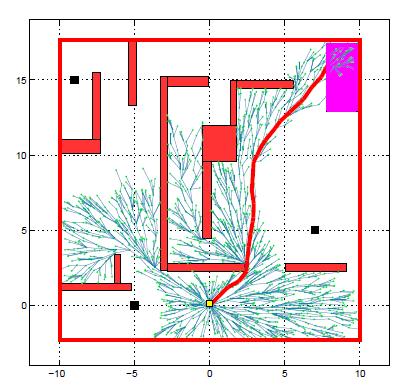
\includegraphics[width=\textwidth]{rrtobs5000}
	\caption{5000 iterations}
	\label{rrtobs5000}
\end{subfigure}
\quad
\begin{subfigure}[b]{0.475\textwidth}
	\centering
	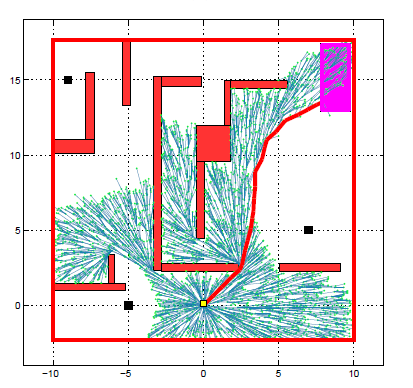
\includegraphics[width=\textwidth]{rrtobs10000}
	\caption{10000 iterations}
	\label{rrtobs10000}
\end{subfigure}
\caption{Pursuit-Evasion $\textnormal{RRT}^*$ in a field with obstacles at various iterations\cite{karaman}}
\label{rrtobsfig}
\end{figure}

\begin{figure}
\centering
\begin{subfigure}[b]{0.475\textwidth}
	\centering
	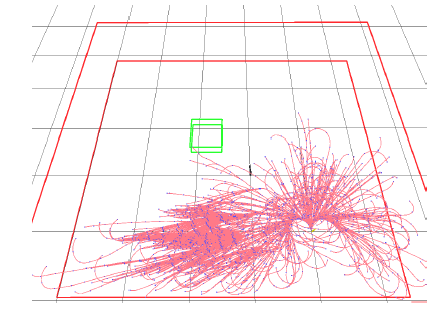
\includegraphics[width=\textwidth]{rrtdubins}
	\caption{Pursuit-Evasion $\textnormal{RRT}^*$ run for 3000 iterations}
	\label{rrtdubins}
\end{subfigure}
\hfill
\begin{subfigure}[b]{0.475\textwidth}
	\centering
	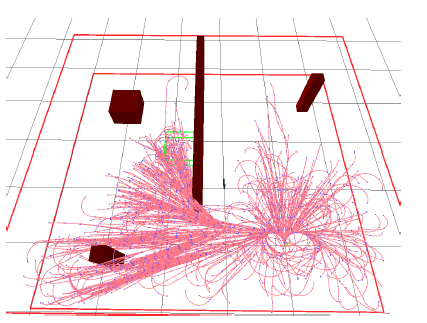
\includegraphics[width=\textwidth]{rrtobsdubins}
	\caption{Pursuit-Evasion $\textnormal{RRT}^*$ run for 3000 iterations in a field with obstacles}
	\label{rrtobsdubins}
\end{subfigure}
\caption{Pursuit-Evasion $\textnormal{RRT}^*$ on a problem with Dubins dynamics \cite{karaman}}
\label{rrtdubinsfig}
\end{figure}

Just as with dynamic programming, there are numerous advantages and disadvantages to using $\textnormal{RRT}^*$ to solve pursuit-evasion games. The computational speed of $\textnormal{RRT}^*$ is the biggest advantage to using this algorithm. 10000 iterations of the simple dynamics example were computed in about 3 seconds, while 3000 iterations of the Dubins dynamics example were computed in about 20 seconds \cite{karaman}. Unlike the dynamic programming method presented in \Cref{1dbvp}, $\textnormal{RRT}^*$ also handles obstacles very well as can be seen in \Cref{rrtobsfig,rrtobsdubins}. 

The major disadvantage of $\textnormal{RRT}^*$-based method is that it computes an open-loop solution. If either the pursuer or evader ends up taking suboptimal actions, the results of the $\textnormal{RRT}^*$ algorithm could be completely useless. For example, suppose that the evader moves into the region of potential pursuer capture by accident. However, the pursuer is elsewhere expecting evader optimal control. In this case the only way to determine a new path for the evader is to recompute the entire solution. Even when the solution is recomputed, it is suboptimal in the feedback sense.             